



\appendix
\section*{Appendix Overview}
\noindent The appendix is organized as follows:\\
\textbf{Section A}: Details of generative pipeline for the \dataset{} dataset.\\
\textbf{Section B}: Statistics of \dataset{} dataset, license for data release and annotator details.\\
\textbf{Section C}: Experimental setup and implementation details.\\
\textbf{Section D}: Additional results from evaluation on the \dataset{} benchmark.\\


\begin{figure*}[t]
    \centering
    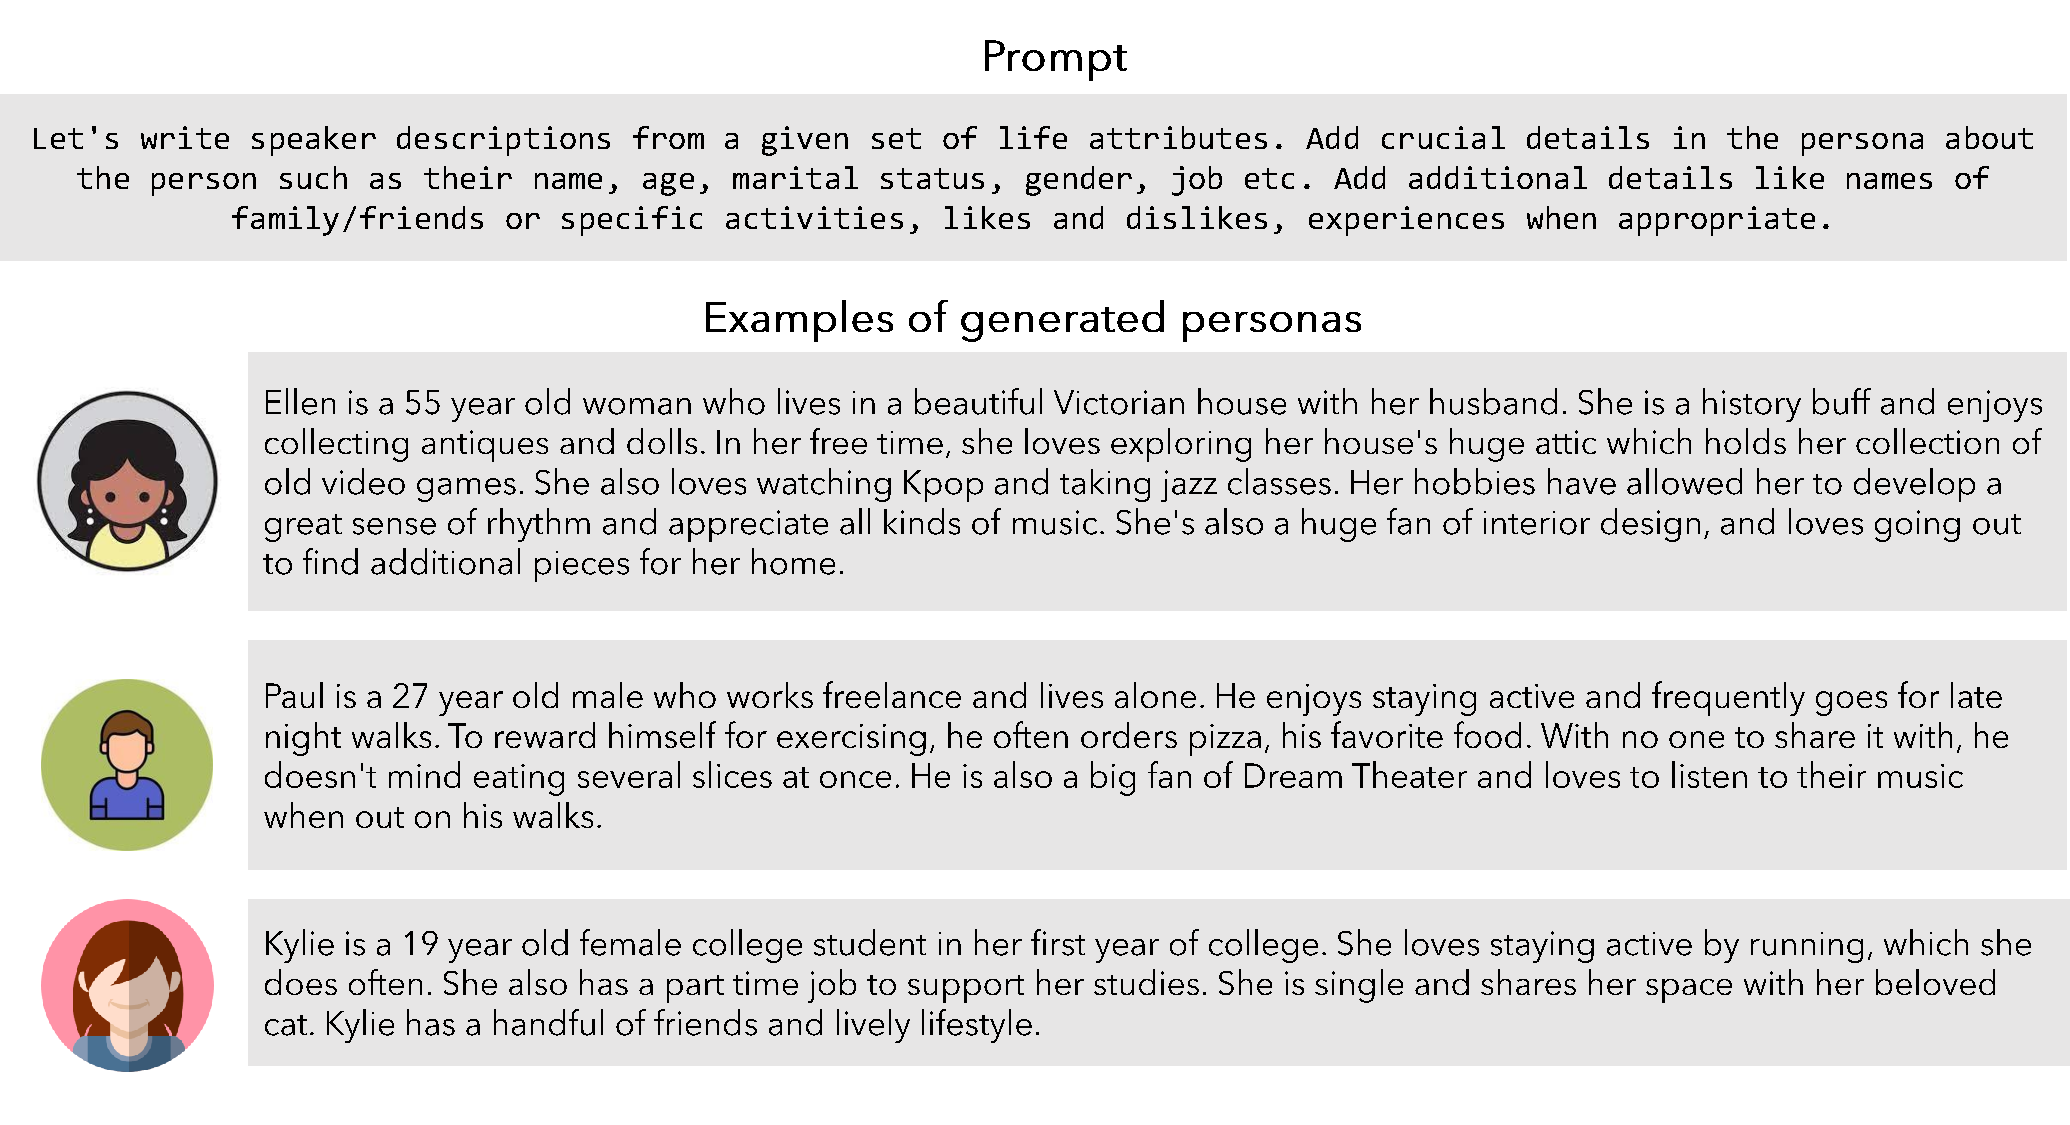
\includegraphics[width=0.99\textwidth]{figures/persona_appendix.pdf}
    \vspace{-10pt}
    \caption{\textbf{Prompt for persona statement ($p$) generation and examples of personas in \dataset{}.} The prompt used to generate expanded persona statements ($p$) from initial personas ($p_c$) for the virtual agents in our conversation generation pipeline (top) and select examples of persona statements present in the \dataset{} dataset.\label{fig:persona}}
\end{figure*}

\section{Generative Pipeline for \dataset{}}
\label{sec:generative-pipeline-appendix}

\subsection{Persona}
\label{ssec:persona_appendix}
We assign unique persona statement $p$ to each agent $\mathcal{L}_i$. For this, we select a range of initial persona statements $p_c$ from the MSC dataset~\cite{xu2022beyond}, each encompassing 4 to 5 sentences. We employ \texttt{gpt-3.5-turbo} as $\mathcal{M}$ to expand these into full persona statement $p$, conditioning $\mathcal{M}$ on the chosen statements $p_c$. The prompt used for converting a short list of speaker attributes from the MSC dataset \cite{xu2022beyond} into a complete persona summary is presented in Fig.~\ref{fig:persona}. We also use a single example of speaker attribute $\rightarrow$ persona summary as an in-context demonstration along with the prompt. A small selection of personas showcasing the diversity of speakers in the \dataset{} dataset is demonstrated in Fig.~\ref{fig:persona}.


\subsection{Temporal Event Graph}
\label{ssec:event_appendix}

\begin{figure*}[t]
    \centering
    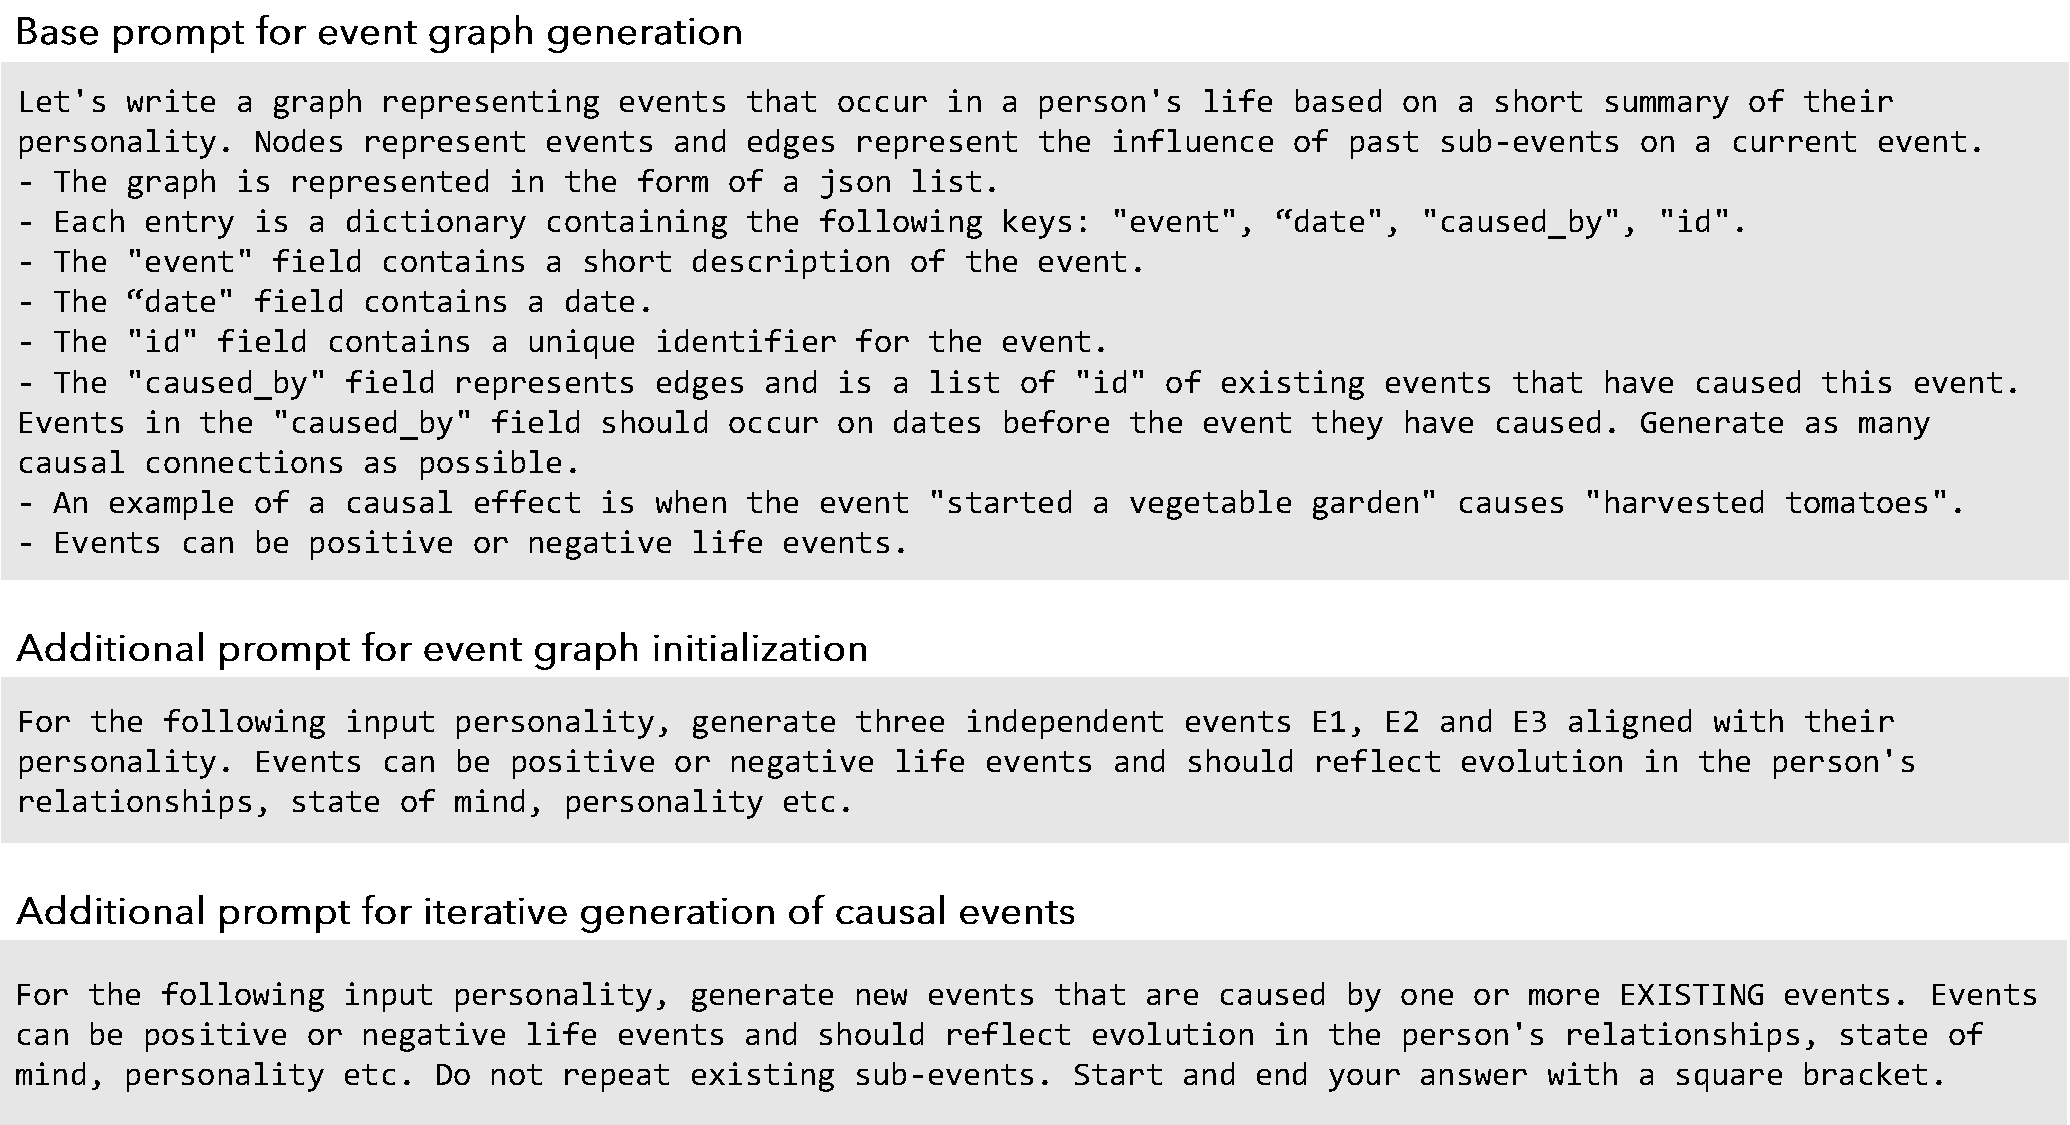
\includegraphics[width=0.99\textwidth]{figures/event_prompts_appendix.pdf}
    \caption{\textbf{Prompts for temporal event graph generation.} The prompt used to generate complete personas for the LLMs in our conversation generation pipeline (top) and examples of personas present in the \dataset{} dataset.\label{fig:event_prompt}}
\end{figure*}


\begin{figure*}[t]
    \centering
    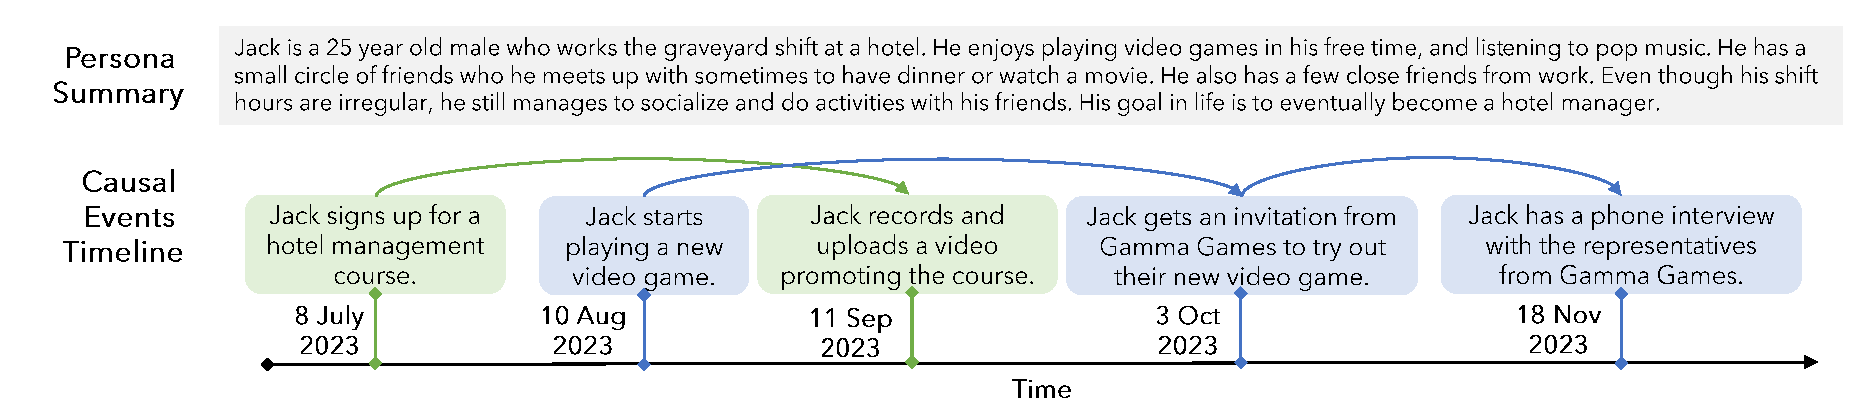
\includegraphics[width=0.99\textwidth]{figures/events.pdf}
    \vspace{-0.5cm}
    \caption{\textbf{Temporal Event Graph $\mathcal{G}$ Creation.} Each event is generated in accordance with the specified persona $p$ and causal connections $l$ between events are depicted to illustrate the casual relationships among them.}
    \label{fig:temporal-event}
\end{figure*}

As outlined in Sec.~\ref{ssec:temporal-event}, we use an iterative process for generating event graphs consisting of causally connected events based on a given persona summary. The base prompt for describing the constitution of the event graph, the nature of events and causal connections between events is shown in Fig.~\ref{fig:event_prompt}. First, the base prompt is used along with the prompt for event graph initialization to generate three independent events relevant to a given personality. Then, the base prompt is combined with the prompt for the iterative generation of events to continue generating events that are caused by one or more of the events that are already present in the graph. See an example of a persona and the corresponding temporal event graph in Fig.~\ref{fig:temporal-event}. In the example, Jack aspires to be a hotel manager. Consequently, he enrolls in a hotel management course in July, and after three months, he expresses his excitement about the course on social media. In a similar vein, his passion for gaming results in an invitation from a well-known gaming company.

\subsubsection{Virtual Agent Architecture}
\label{sssec:agent_appendix}

As outlined in Section~\ref{ssec:llm-agent}, the virtual agents in our generative pipelines are composed of two mechanisms, \textit{Reflect \& respond} \cite{park2023generative} and \textit{Image sharing \& response}.

\paragraph{Reflect \& respond.} This mechanism operates over a combination of short-term and long-term memory. The short-term memory is a summary of a session that is conditioned on the summary from a previous session. See the prompt given to LLMs in our pipeline for generating summaries, and an example of a generated summary, in Fig.~\ref{fig:summary_prompt}. The long-term memory is a database of \textit{observations} about each speaker, that are essentially assertive statements about the speaker's persona and life. See the prompt given to LLMs in our pipeline for generating observations, and an example of observations extracted from a conversation, in Fig.~\ref{fig:observation_prompt}. In practice, the conversation is annotated with turn IDs for each turn, and the model is also instructed to indicate the turn IDs that directly contribute to each observation. This allows us to keep track of the evidence when using observations as the context for RAG-based models used in our experiments (see Section~\ref{sec:baselines}).

\paragraph{Image sharing \& response.} See prompts for implementing image-sharing and image-response behaviors in Figure~\ref{fig:image_prompt}. 

\begin{figure*}[t]
    \centering
    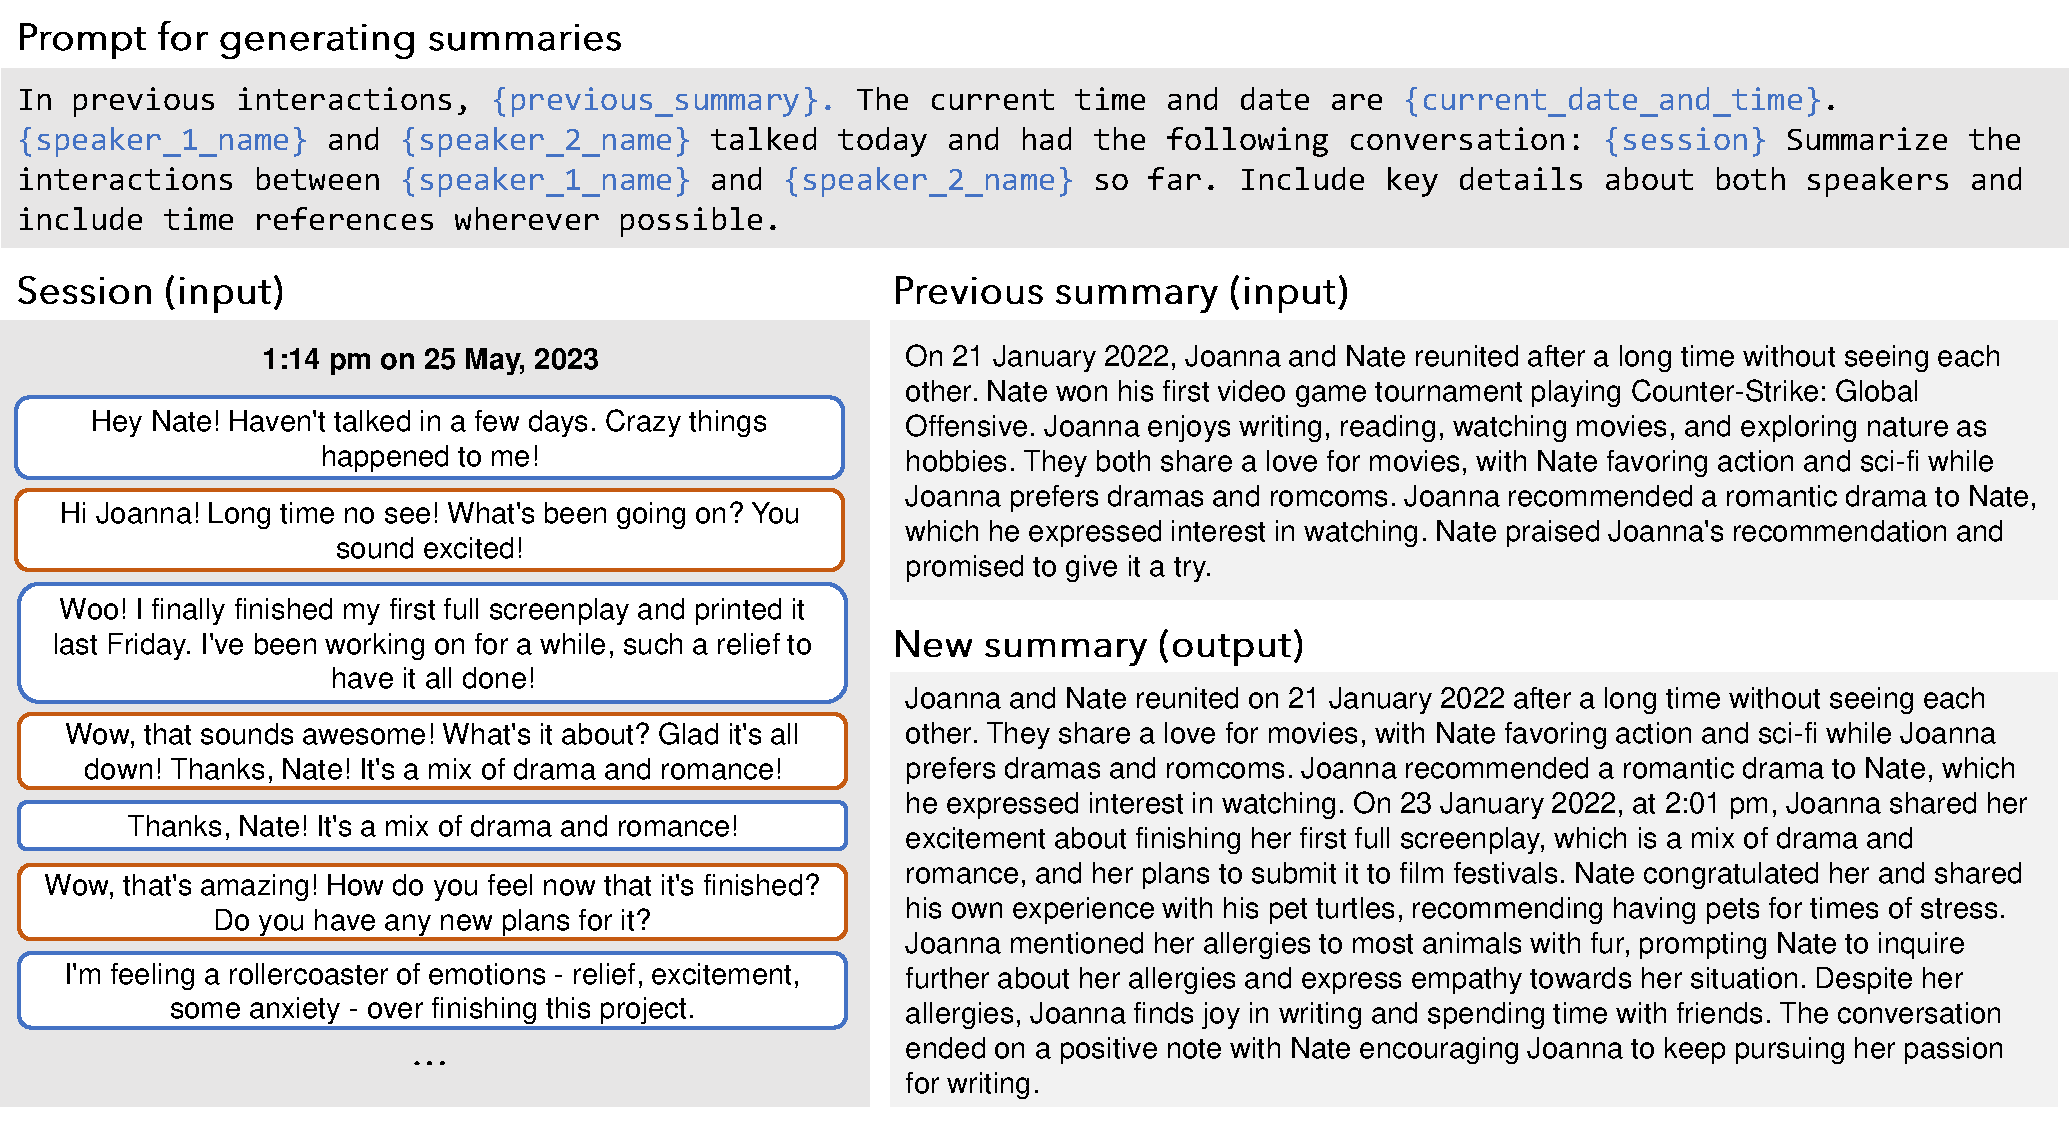
\includegraphics[width=0.99\textwidth]{figures/summary_prompt_arxiv.pdf}
    \caption{\textbf{Prompt for generating conversation summaries.} The prompt used to iteratively generate a summary for the current session by conditioning on summary from preceding sessions and the raw conversation logs of the current session (top); and an example of inputs for the prompt and corresponding output summary of a session from the \dataset{} dataset. \label{fig:summary_prompt}}
\end{figure*}

\begin{figure*}[t]
    \centering
    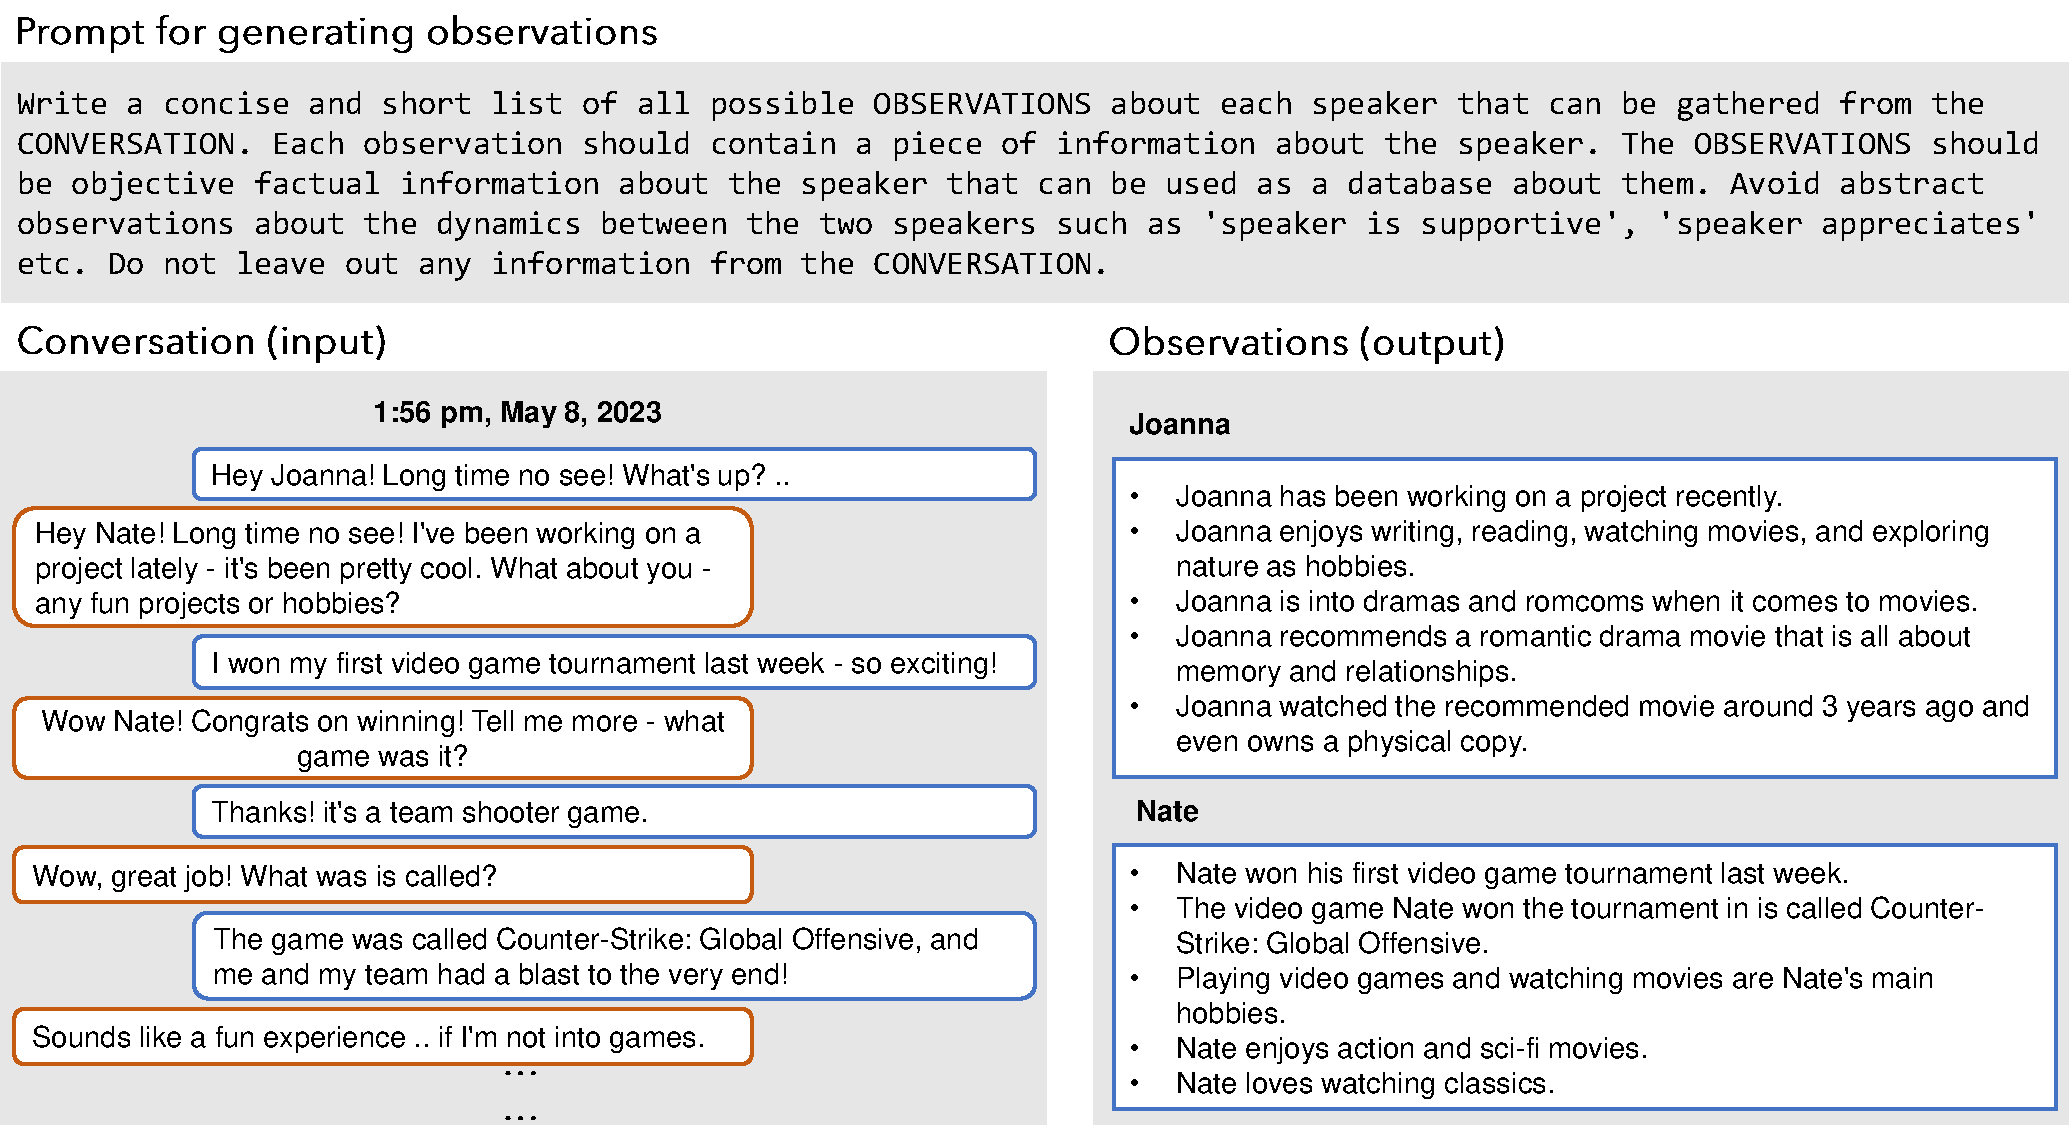
\includegraphics[width=0.99\textwidth]{figures/observation_prompt_arxiv.pdf}
    \caption{\textbf{Prompts for generating observations from conversations.} The prompt used to generate observations from a conversation (top); and an example of inputs for the prompt and corresponding output observations for a session from the \dataset{} dataset.\label{fig:observation_prompt}}
\end{figure*}

\begin{figure*}[t]
    \centering
    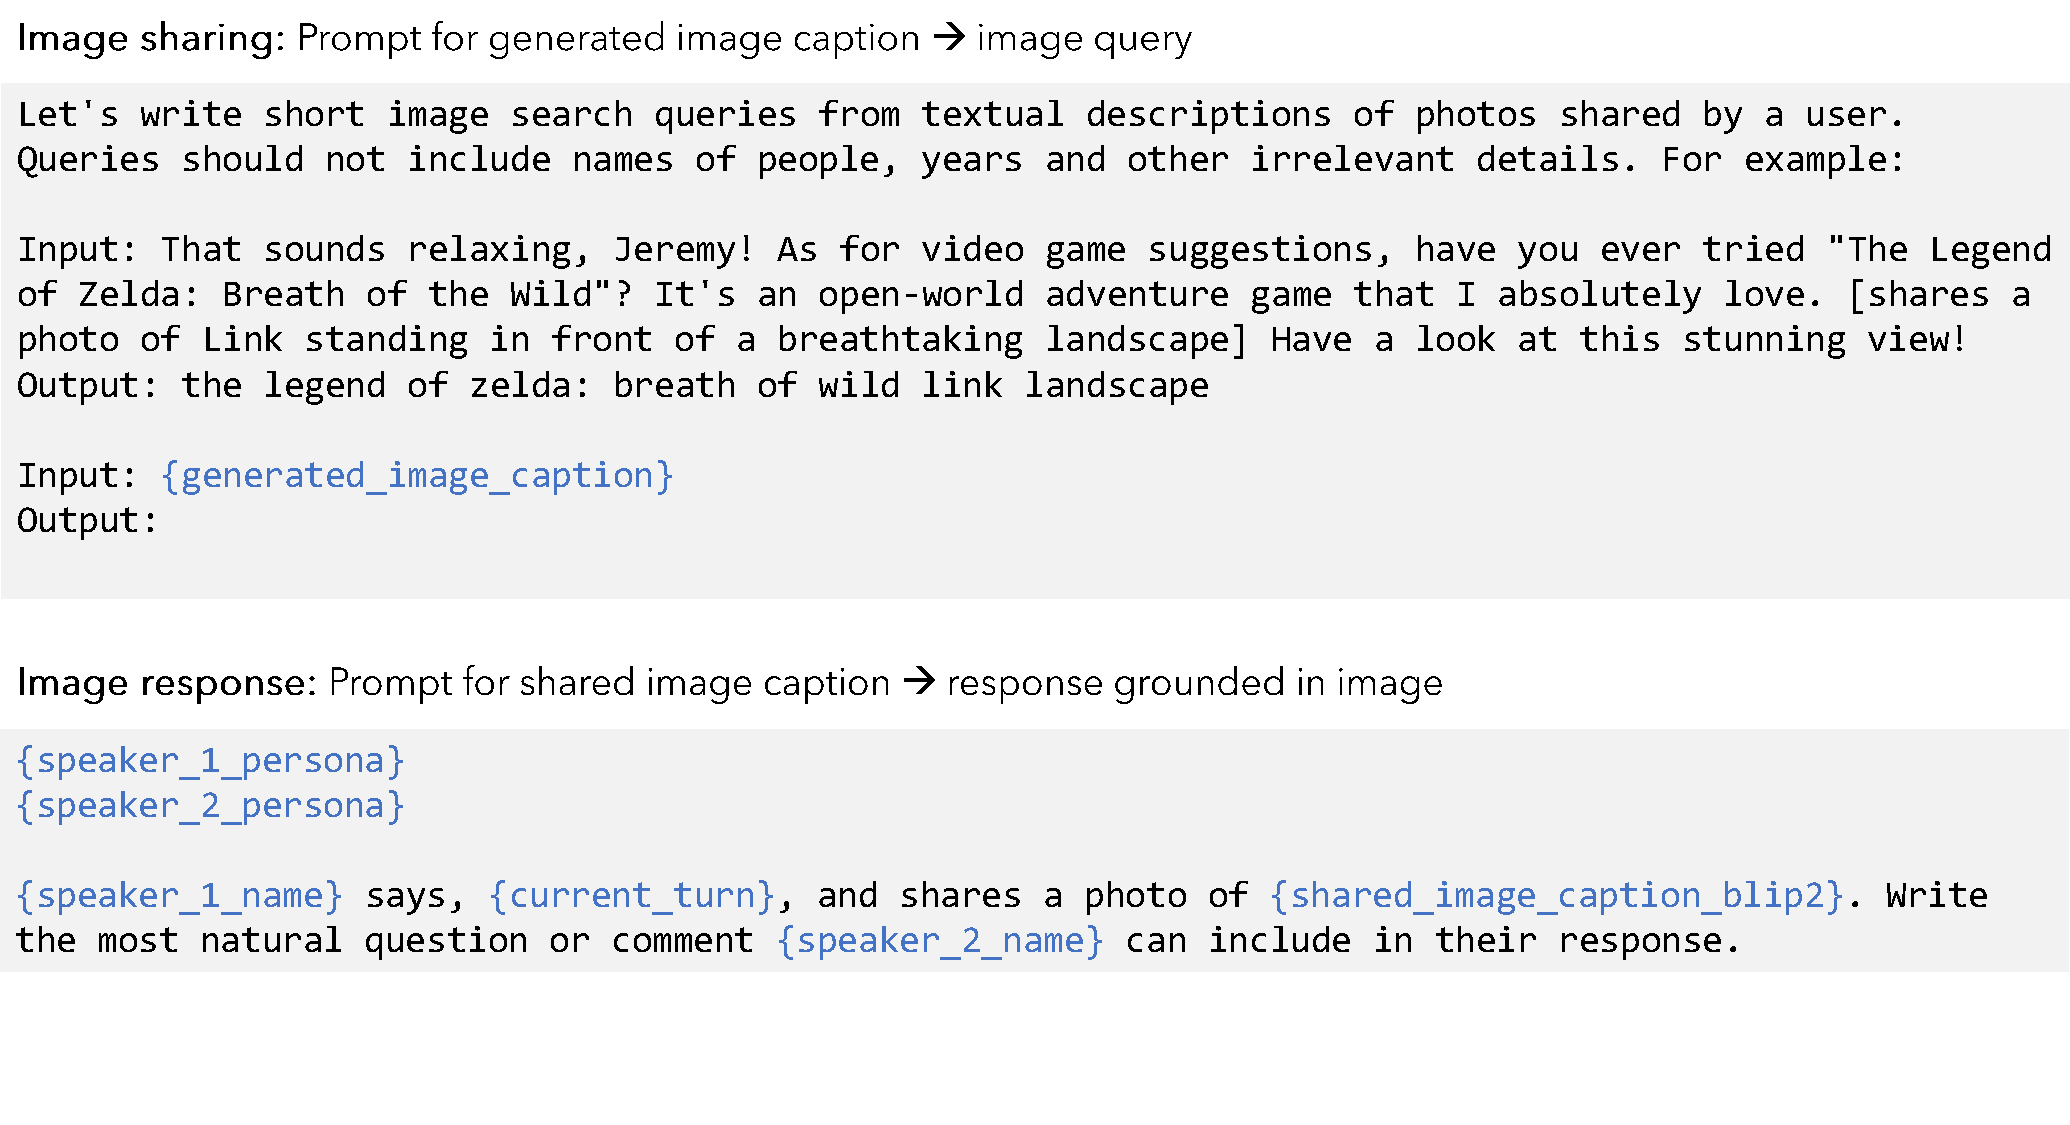
\includegraphics[width=0.99\textwidth]{figures/image_prompts.pdf}
    \vspace{-30pt}
    \caption{\textbf{Prompts for image-sharing and image-response behavior.} The prompt used to convert a caption generated by the virtual agent into an image query for the web-based image crawler in our pipeline (top), and the prompt used to generate a response grounded in the image shared by a virtual agent during a conversation as well as the personas of the respective speakers (bottom).\label{fig:image_prompt}}
\end{figure*}


\subsection{Human Filtering}
\label{ssec:edits_appendix}

\begin{figure*}[t]
    \centering
    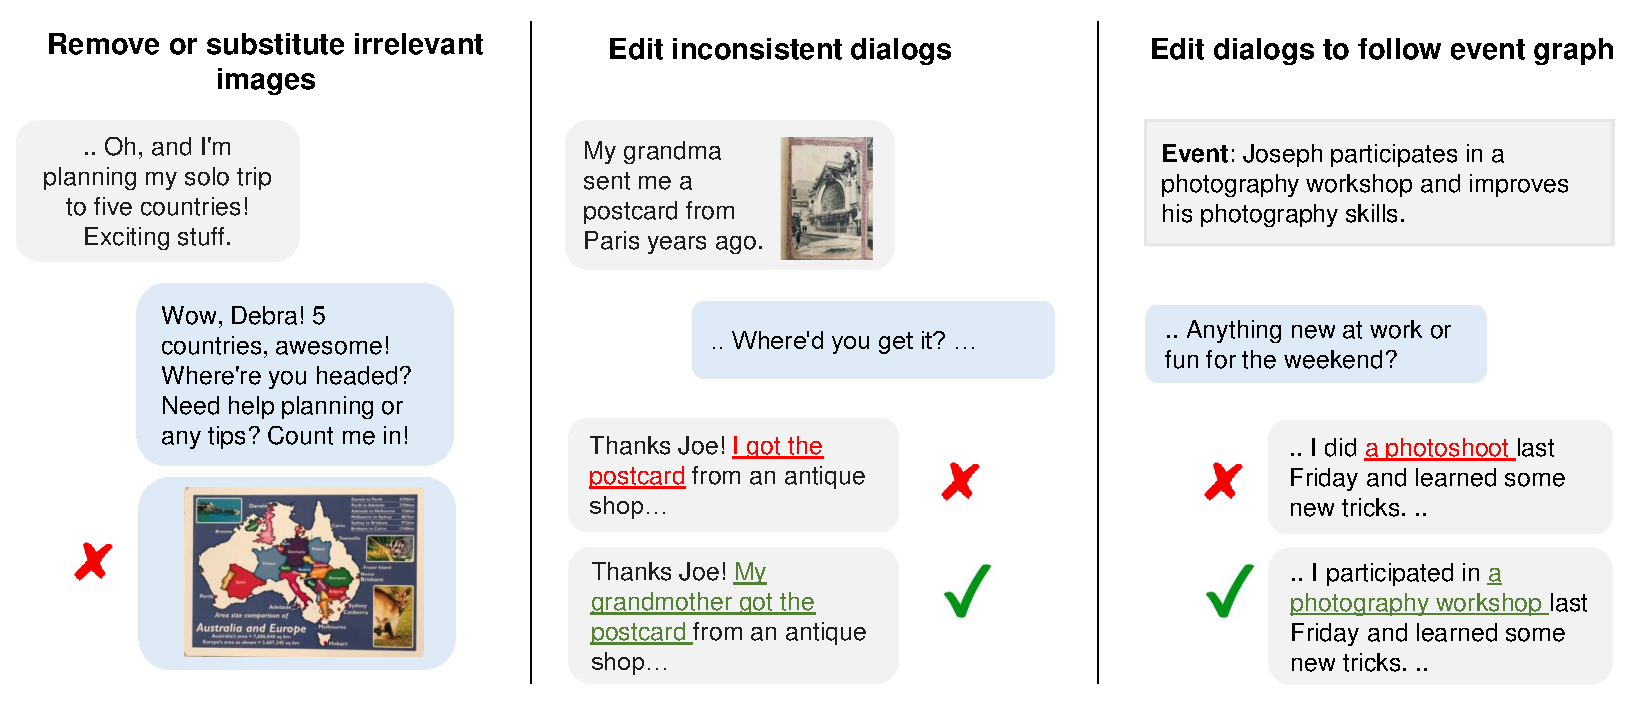
\includegraphics[width=0.99\textwidth]{figures/conv_edits.pdf}
    \caption{\textbf{Example of edits made by annotators.} Human annotators are instructed to make edits in the LLM-generated conversations to remove irrelevant The prompt used to generate complete personas for the LLMs in our conversation generation pipeline (top) and examples of personas present in the \dataset{} dataset.\label{fig:conv_edits}}
\end{figure*}


Human annotators are instructed to edit the LLM-generated conversations in the following scenarios:
\begin{itemize}
    \item Remove an image if it is not relevant to the current dialog or the conversation.
    \item Add context about an image to the current speaker's dialog if it is not discussed by them but the subsequent speaker has reacted to the image.
    \item Replace an image if it does not match the caption that was used to query for images.
    \item Edit the dialog when the information present in the dialog is inconsistent with something said (or shared through an image) in earlier or later turns.
    \item Edit the dialog to ensure that the details in the conversation are consistent with those given in the event for the session.
    \item Remove any events from the event graph if they do not appear in the conversation.
\end{itemize}

See an example of some edits in Fig.~\ref{fig:conv_edits}.

\section{Dataset}

\subsection{Dataset Statistics}
See a breakdown of the statistics of the conversations in the \dataset{} dataset in the top panel of Table~\ref{tab:dataset_statistics}. Also, see a breakdown of the statistics of the annotations in the evaluation benchmark in the bottom panel of Table~\ref{tab:dataset_statistics}.

\begin{table}[t]
	\centering
	\small
	\resizebox{\linewidth}{!}{
		\begin{tabular}{lc}
            \toprule
            \rowcolor{gray!20} Conversation Statistics & \# Counts \\
            \midrule
             Total. \# conversations $h$. & 50 \\
             Avg. \# sessions $k$. in conversation $h$ & 19.3 \\
             Avg. \# turns $j$. in session $k$ & 15.8 \\
            \midrule
             Avg. \# tokens. conversation $h$ & 9,209.2 \\
             Avg. \# tokens. dialogue $h_{k_j}$ of turn $j$ in session $k$ &  30.2 \\
             Avg. \# tokens. observation $o_{k_j}$ of turn $j$ in session $k$ & 18.2 \\
             Avg. \# tokens. summary $w_k$ of session $k$ & 127.4 \\
             \midrule
             \rowcolor{gray!20} QA Benchmark Statistics & \\
             \midrule
             \# questions. single-hop retrieval & 2,705 (36\%)\\
             \# questions. multi-hop retrieval & 1,104 (14.6\%)\\
             \# questions. temporal reasoning &  1,547 (20.6\%)\\
             \# questions. open domain knowledge & 285 (3.9\%)\\
             \# questions. adversarial & 1,871 (24.9\%)\\
             \textbf{Total. \# questions.} & \textbf{7,512} \\
             \midrule
             \rowcolor{gray!20} Event Summarization Statistics & \\
             \midrule
             Avg. \# ground truth events. in conversation $h$ & 24.2 \\
             Avg. \# tokens. event summary & 896.5 \\
             \midrule
             \rowcolor{gray!20} Multi-modal Dialogue Generation Statistics & \\
             \midrule
             Avg. \# images. in conversation $h$ & 32.3 \\
            \bottomrule
        \end{tabular}
	}
        \caption{\textbf{Dataset Statistics} of conversation and corresponding benchmark}
	\label{tab:dataset_statistics}
\end{table}

\subsection{Dataset License}
The \dataset{} dataset will be released under the CC BY-NC 4.0 DEED license.\footnote{\url{https://creativecommons.org/licenses/by-nc/4.0/}}

\subsection{Annotator Details}
The annotators who worked on the \dataset{} dataset were in-house annotators and we were unable to obtain their demographics due to the confidential nature of such information.

\section{Experimental Setup}
\label{sec:experiments_appendix}

\subsection{Baselines}
\label{ssec:baselines-appendix}
The conversations in the \dataset{} dataset are composed of natural language dialogs and images that require higher-order reasoning and multimodal coreference resolution, respectively. From initial studies, we observed that multimodal coreference resolution can be performed effectively by replacing images in \dataset{} with their captions generated using BLIP-2 \cite{li2023blip}, and using state-of-art LLMs to reason over natural language text interleaved with image captions. Hence, our experiments for the question answering and event summarization tasks are conducted using LLMs. We use the images directly only for experiments on the multimodal dialog generation task.

\paragraph{Question Answering.}
We carry out experiments using three distinct methodologies:
(1) \textbf{Base} involves utilizing LLMs to directly conduct the task within a constrained context.
The task description comes after the dialogue history. 
To accommodate the restricted context window size, earlier dialogues are omitted; 
(2) \textbf{Long-context} employs LLMs with an extended context window to expose the models to as much dialogue context as possible;
(3) \textbf{Retrieval-augmented Generation (RAG)} involves retrieving relevant context from a database of dialog history, observations, or session-level summaries. \textit{Observations} are assertions about each speaker extracted from the dialog history as described in \Sref{ssec:llm-agent}, see an example in Figure~\ref{fig:observation_prompt}. Session-level \textit{summaries} are concise summaries of the conversation that takes place in each session, see an example in Figure~\ref{fig:summary_prompt}.

For the retrieval model, we employ DRAGON~\cite{lin-etal-2023-train}.
In the \textit{Base}, we utilize Mistral-7B~\cite{jiang2023mistral}, LLama-70B-chat~\cite{touvron2023llama}, \texttt{gpt-3.5-turbo}~\footnote{https://platform.openai.com/docs/models/gpt-3-5}, and \texttt{gpt-4-turbo}~\footnote{https://platform.openai.com/docs/models/gpt-4-and-gpt-4-turbo}. 
To assess the effectiveness in practical scenarios for \textit{Long-context} and \textit{RAG}, we draw comparisons using variants of \texttt{gpt-3.5-turbo}.
We do not report the performance of long-context fine-tuned open-source models~\cite{chen2023longlora} or those utilizing sliding window~\cite{bertsch2024unlimiformer, dao2022flashattention} due to the variability inherent across different open-source models and the potential reduction in their capability on shorter context.

\paragraph{Event Summarization.}
We present experiments conducted in two distinct configurations.
We use both the \textbf{Base} and \textbf{Long-context} setups from the question answering task, but we refrained from including RAG since summarization requires a comprehensive understanding of the entire dialogue, rather than just retrieving a specific portion. A notable distinction in our approach, compared to the question-answering task, lies in our handling of the context. 
Specifically, we employ an iterative process of creating a summary of a preceding session and then use that summary as a basis to generate the summary for the subsequent session \cite{chang2023booookscore}. Further, we use a single in-context demonstration of input and output to guide the model toward selecting only significant life events for the summary.

\paragraph{Multi-modal Dialogue Generation.}
For evaluating multi-modal dialogue generation, we train MiniGPT-5~\cite{zheng2023minigpt} on 50 conversations generated using our automated pipeline (without human filtering) as detailed in \Sref{sec:dataset}.
Three distinct versions of the model were developed, each with varying training data:
(1) \textbf{Base} trains on preceding dialogue turns;
(2) \textbf{+ summary} trains on both prior dialogue turns and a global summary of the ongoing conversation;
(3) \textbf{+ observation} trains on both preceding dialogue turns and relevant observations retrieved from the conversation history.
For each of these models, we started with a MiniGPT-5 checkpoint pretrained on the MMDialog dataset \cite{feng2023mmdialog}.

\subsection{Implementation Details}
We use OpenAI API and Huggingface~\cite{wolf-etal-2020-transformers}, as of January 2024, with specific settings of $temperature$ set to 0 and $top_p$ set to 1 for evaluation of the \dataset{} benchmark. All experiments, including those for RAG-based models, MiniGPT-5 training, and inference, are conducted on an Nvidia A6000 server with FP32. We report results from a single inference run for each model in our experiments. For MiniGPT-5, we used the hyperparameters recommended in the original codebase and trained our models for 10 epochs, which took approximately 30 hours on a single A6000 GPU.

We use the default implementations of BLEU\footnote{\url{https://www.nltk.org/_modules/nltk/translate/bleu_score.html}}, ROUGE\footnote{\url{https://pypi.org/project/rouge/}}, BertScore\footnote{\url{https://pypi.org/project/bert-score/}}, FactScore\footnote{\url{https://github.com/shmsw25/FActScore}} metrics in their respective Python packages in our evaluation protocol.

\section{Results}

\begin{table}[t!]
	\centering
	\small
	\resizebox{\linewidth}{!}{
		\begin{tabular}{ccccc}
            \toprule
             \textbf{Category} & \textbf{top-$k$} & \textbf{BLEU-1/2} & \textbf{Rouge-L} & \textbf{MM-R} \\
            \midrule
                \texttt{Base}  &  - & 57.1 / 34.2 & 12.4 & 56.1 \\
            \midrule
                \texttt{+ summary} & \cellcolor{gray!30} 1 & 58.2 / 34.1 & 12.8 & 56.9 \\
                \texttt{+ summary} & \cellcolor{gray!45} 2 & 56.5 / 32.8 & 12.1 & 55.1 \\
                \texttt{+ summary} & \cellcolor{gray!60} 5 & 56.1 / 32.5 & 12.0 & 55.2 \\
            \midrule
                \texttt{+ observation} & \cellcolor{gray!30} 5 & \textbf{59.7} / \textbf{35.1} & \textbf{13.6} & \textbf{57.8} \\
                \texttt{+ observation} & \cellcolor{gray!45} 10 & 59.1 / 34.9 & 12.8 & 57.1 \\
                \texttt{+ observation} & \cellcolor{gray!60} 25 & 58.5 / 34.2 & 12.0 & 56.5 \\
            \bottomrule
        \end{tabular}
	}
        \caption{\textbf{Multi-modal dialogue generation performance} comparison between different training variants of MiniGPT-5.
        The optimal performance is shown in \textbf{bold}.}
	\label{tab:dialog_results}
\end{table}



\subsection{Event Summarization Task}
\label{ssec:appendix-event-summ}

See an example of the five broad categories of event summarization errors made by LLMs, outlined in Section~\ref{ssec:event-results}, in Table~\ref{tab:summary_errors}.

\begin{table*}[t!]
	\centering
	\small
	\resizebox{\linewidth}{!}{
		\begin{tabular}{P{0.7in}>{\columncolor{blue!10}}P{2.2in}>{\raggedright}P{2.8in}P{1.8in}}
            \toprule
             \textbf{Error Type} & \textbf{Explanation} & \textbf{Ground truth event \textit{or} relevant dialogs} & \textbf{Predicted event} \\
            \midrule
            Missing information & Key details about event are omitted because the model fails to make causal and temporal connections over a long conversation. & Joanna submits her third screenplay on loss, identity, and connection to a film contest & Joanna submits her recent screenplay to a film contest. \\
            \midrule
            Hallucination & Non-existent details or details from a different event are padded onto an event & \textit{N}: `The gaming party was a great success!' \newline \textit{N}: `... said they'd want to do it again next month!' \newline \textit{N}: `On another note, I made vegan ice cream ...' & Nate's vegan ice cream is a huge success and people want to do it again next month. \\
            \midrule
            Misunder- -standing of dialog cues & e.g., model confuses a light-hearted statement from a speaker as a serious statement & \textit{J}: `.. these trails that made me feel like writing a drama.' \newline \textit{N}: `.. go together .. Maybe I'll start to think of a drama myself and write a screenplay ...' \newline \textit{J}: `Haha, now that would be something! ...' & Nate considers writing his own drama screenplay. \\
            \midrule
            Speaker attribution & Event is attributed to the wrong speaker & Nate invites Joanna to try his homemade lactose-free ice cream. & Joanna invites Nate to her home to try her dairy-free ice cream recipe. \\
            \midrule
            Saliency & Unimportant interactions in the conversation are considered significant by model & \textit{N}: Hey Joanna, what's been up since we last chatted? How's it going? & Nate asks Joanna how she has been she they last talked.\\
            \bottomrule
        \end{tabular}
	}
        \caption{\textbf{Taxonomy of errors in LLM-generated event summaries.} Five types of errors predominantly occur in the event summaries generated by LLMs. Examples are based on predictions from \texttt{gpt-3.5-turbo}.}
	\label{tab:summary_errors}
\end{table*}

\subsection{Multimodal Dialog Generation Task}


Results from evaluation of various version of MiniGPT-5 model on the multimodal dialog generation task in the \dataset{} benchmark is in Table~\ref{tab:dialog_results}.


